\documentclass{beamer}

\mode<presentation> { \usetheme{gruvbox} }
\setbeamerfont{frametitle}{size=\huge}


\usepackage{graphicx} % Allows including images
\usepackage{booktabs} % Allows the use of \toprule, \midrule and \bottomrule in tables
%\usepackage{listings}             % Include the listings-package
\usepackage{minted}
\usepackage{tikz}
\usepackage{drawstack}
\usetikzlibrary{calc,shapes.callouts,shapes.arrows,chains,positioning,fit,shapes, arrows.meta, arrows}
\usepackage{verbatimbox}
\usepackage{tcolorbox}
\usepackage{forloop}
\usepackage{seqsplit}
\usepackage{bytefield}


\hypersetup{
    colorlinks=true,
}
\usemintedstyle{paraiso-dark}
\graphicspath{ {./images/}{../../slides-source-dep/images/} }
\DeclareGraphicsExtensions{.png,.pdf}

\newcommand{\pointthis}[2]{
    \tikz[remember picture,baseline]{\node[anchor=base,inner sep=0,outer sep=0]%
    (#1) {\underline{#1}};\node[overlay,rectangle callout,%
    callout relative pointer={(0.2cm,0.7cm)},fill=green!50] at ($(#1.north)+(-.5cm,-1.4cm)$) {#2};}%
}%

\newcounter{loopcntr}
\newcommand{\rpt}[2][1]{%
  \forloop{loopcntr}{0}{\value{loopcntr}<#1}{#2}%
}

\newcommand{\hash}[1]{{\ttfamily\seqsplit{#1}}}

\newlength{\bitlabelwidth}
\newcommand{\rotbitheader}[1]{%
  \tiny
  \settowidth{\bitlabelwidth}{\quad 9999}%
  \rotatebox[origin=B]{60}{\makebox[\bitlabelwidth][r]{#1}}%
}

\newenvironment{zerohyphen}
 {\global\chardef\savedhyphenchar=\hyphenchar\font % save the current hyphenchar
  \lefthyphenmin=1 \righthyphenmin=1 % no limits on hyphenation
  \hyphenchar\font=23 }
 {\par\hyphenchar\font=\savedhyphenchar}% eject the paragraph and restore

%----------------------------------------------------------------------------------------
%	TITLE PAGE
%----------------------------------------------------------------------------------------

\title[Introduction to Binary Exploitation]{\huge \textbf{Introduction to Binary Exploitation}} % The short title appears at the bottom of every slide, the full title is only on the title page

\author{Andrew Haberlandt} % Your name
\date{Feburary 23, 2021} % Date, can be changed to a custom date

\begin{document}

{ % this brace groups the background template with just the first slide
\usebackgroundtemplate{%
    \begin{tikzpicture}
        \path [outer color = blue!5, inner color = blue!1]
        (0,0) rectangle (\paperwidth,\paperheight);
        \node[anchor=south west, inner sep=0,line width=0,draw,text width=\paperwidth,fill=almostblack] at (0,0) {\textcolor{darkgray}{\hash{00110110100011010001101101101111100010010111011001110101001111101110100101100101001000001010111000001100110000111010100100001110100010110101001010100001011100000110011111111111100110011010100100101111110111110011101011110010100001001101101010111111011000010110011101110110110000000101101101111110111010111001110010111100110110100100111110111011010110111010101101000011000100011101001011010101111101010000001000001111011111000100111001010000101010000010111001101111101111011111011001110100101101100000011000011110110111010111110001111001110011011110101001001011110001101010110000110110100011000101110110101001110100011101100111101000001001111110000111100010010110000111110101010100000000001110000001010001110110001111000100001100010110101011100011101110101100111111010111101000100111000011110110100011000110111011001101101111111100001010101010010100100101110101011111010110100111011000101010111000010110010010011000010110011000111000110110000010110001100110100011000000111100110110101011100100011110100011011010001101000110110110111110001001011101100111010100111110111010010110010100100000101011100000110011000011101010010000111010001011010100101010000101110000011001111111111110011001101010010010111111011111001110101111001010000100110110101011111101100001011001110111011011000000010110110111111011101011100111001011110011011010010011111011101101011011101010110100001100010001110100101101010111110101000000100000111101111100010011100101000010101000001011100110111110111101111101100111010010110110000001100001111011011101011111000111100111001101111010100100101111000110101011000011011010001100010111011010100111010001110110011110100000100111111000011110001001011000011111010101010000000000111000000101000111011000111100010000110001011010101110001110111010110011111101011110100010011100001111011010001100011011101100110110111111110000101010101001010010010111010101111101011010011101100010101011100001011001001001100001011001100011100011011000001011000110011010001100000011110011011010101110010001111010}}};
    \end{tikzpicture}
}


\begin{frame}
    \titlepage % Print the title page as the first slide
    \begin{tikzpicture}[overlay]
        \node[anchor=south east, yshift=-1cm, xshift=-2cm] (shirt1) at (current page.south east) {
\includegraphics[width=0.15\paperwidth]{logo.png}};
    \end{tikzpicture}
    \begin{itemize}
        \item \textbf{Don't forget to start recording}
        \item Slides are on https://wiki.osucyber.club
        \item \small{Some content adapted from: Nathan Peercy (Purdue)}
    \end{itemize}
\end{frame}
} % end background template


\begin{frame}
    \frametitle{Announcements}
    \begin{itemize}
        \item \textbf{Next Week:} Group solve time focusing on pwn
    \end{itemize}
\end{frame}


\setbeamercolor{background canvas}{bg=almostblack}
\setbeamertemplate{section in toc}[square]
\begin{frame}
    \frametitle{Overview} % Table of contents slide, comment this block out to remove it
    \tableofcontents % Throughout your presentation, if you choose to use \section{} and \subsection{} commands, these will automatically be printed on this slide as an overview of your presentation
\end{frame}


\section{What is binary exploitation?}
\begin{frame}
    \frametitle{What is binary exploitation?}
    \begin{itemize}
        \item{Make a [compiled/binary] program do something it wasn't intended to do}
        \item{Usually this means the goal is arbitrary code execution}
        \item{pwn is awesome but pwn is hard. You'll eventually need a good understanding of:}
        \begin{itemize}
            \item{Assembly}
            \item{C}
            \item{Operating systems}
        \end{itemize}
    \end{itemize}
\end{frame}


\begin{frame}
    \frametitle{Why}
    \begin{itemize}
        \item{Native code is everywhere}
        \item{No really, EVERY APPLICATION EVER ULTIMATELY ENDS UP RUNNING MACHINE CODE}
    \end{itemize}
\end{frame}


\begin{frame}
    \begin{tikzpicture}[overlay]
        \node[anchor=south east, yshift=-5cm, xshift=-4cm] (turtle) at (current page.south east) {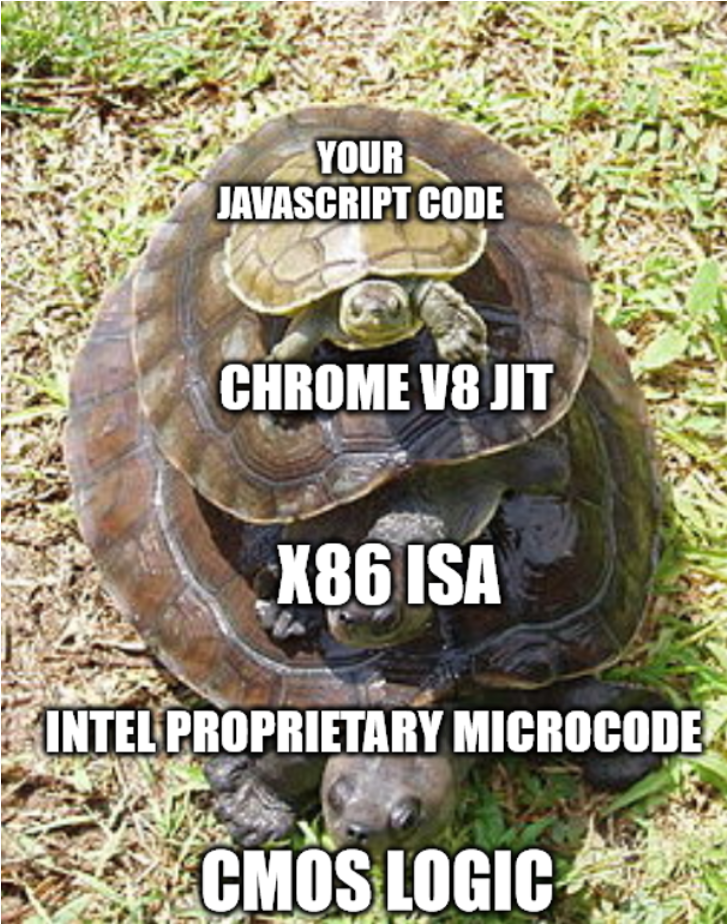
\includegraphics[width=0.5\paperwidth]{turtle.png}};
    \end{tikzpicture}
\end{frame}


\begin{frame}
    \frametitle{Why}
    \begin{itemize}
        \item{GOAL: Take over ('pwn') a machine}
        \begin{itemize}
            \item{If you can run whatever code you want, you can do anything the OS allows that program to do (usually anything the user has access to do)}
            \item{After you have code execution, 'privilege escalation' concerns exploiting (usually) the operating system to gain additional privileges (i.e. normal user -> root access, or sometimes directly to kernel code execution)}
            \item{Some special programs (ie. sudo) are usually given extra privileges to run as root ("suid programs"); exploit one of these and you get insta-root.}
            \item{Bug Bounties: \href{https://hackerone.com/valve?type=team}{Valve}, \href{https://bugcrowd.com/tesla}{Tesla}, many others}
        \end{itemize}
    \end{itemize}
\end{frame}


\begin{frame}
    \frametitle{What does it look like to 'pwn' a machine?}
    \begin{itemize}
        \item{\textbf{Arbitrary code execution}}
        \begin{itemize}
            \item{Often demonstrated by: getting a shell (opens on stdin)}
            \item{"popping calc"}
            \item{Sometimes in CTF problems: opening and reading a special 'flag' file is sufficient (can do with shell, or not)}
            \item{After you have code execution, you're often done unless you're the NSA or CIA}
        \end{itemize}
    \end{itemize}
\end{frame}


\begin{frame}
    \frametitle{Demo 1: Reverse shell in Bash}
\end{frame}


\section{OK, how do I get code execution?}
\subsection{Common vulnerabilities}
\begin{frame}
    \frametitle{Common vulnerabilities}
    \begin{itemize}
        \item{Command injection}
        \item{Memory corruption: a broad category}
        \item{Off-by-one errors}
        \item{Race conditions}
        \item{(lack of) Input validation}
        \item{Miscellaneous logic bugs}
    \end{itemize}
\end{frame}


\subsection{Command Injection}
\begin{frame}
    \frametitle{Command Injection}
\end{frame}


\begin{frame}
    \frametitle{Demo 2: Command injection + pwntools}
\end{frame}


\subsection{Logic Bugs}
\begin{frame}
    \frametitle{Logic Bugs}
    \begin{itemize}
        \item{Most are unintentional, Intentional logic bugs are essentially "backdoors".}
        \item{Leaving in debug options: "bypass this security measure by adding debug=1"}
        \item{Program gets confused about state when receiving packets/commands out-of-order}
        \item{TODO: need more logic bug examples}
    \end{itemize}
\end{frame}


\subsection{Memory Corruption Bugs}
\begin{frame}
    \frametitle{Memory Corruption Bugs}
    \begin{itemize}
        \item{Memory is a byte-addressable array of bytes}
        \item{If a user can write somewhere they are not intended to, it can be the cause of a memory corruption bug}
        \item{The important question is "can we overwrite anything important?"}
        \begin{itemize}
            \item{To answer, need to know some things about where stuff is in memory}
        \end{itemize}
    \end{itemize}
\end{frame}


\begin{frame}
    \frametitle{Simplest example: Stack buffer overflow into another variable}
\end{frame}


\begin{frame}
    \frametitle{More examples: What if we can write anywhere? (Where should we write?)}
\end{frame}


\begin{frame}
    \frametitle{More examples: Semi-arbitrary write (controlled array index)}
\end{frame}


\begin{frame}
    \frametitle{Simple example: Stack buffer overflow into return address}
\end{frame}


\begin{frame}
    \frametitle{1990s exploitation}
    \begin{itemize}
        \item{Just put your code somewhere you know the address of, and then overwrite the return address so that it holds the address of your code}
        \item{When the function returns, you win}
    \end{itemize}
\end{frame}


\begin{frame}
    \frametitle{Demo 3: Return to the 1990s + pwntools}
\end{frame}


\subsection{ROP}
\begin{frame}
    \frametitle{Moden memory protections have entered the chat}
    \begin{itemize}
        \item{You can't just write your code onto the stack and jump to it. The stack is not executable.}
        \item{We need to be more creative}
    \end{itemize}
\end{frame}


\begin{frame}
    \frametitle{ROP}
    \begin{itemize}
        \item{We don't just control the return address, we can keep writing and we control the whole stack}
        \item{We can return to specific locations that do useful things and then come back ('gadgets')}
        \begin{itemize}
            \item{pop rdi; ret;}
        \end{itemize}
        \item{Chain these together and you can make syscalls, etc.}
    \end{itemize}
\end{frame}


\begin{frame}
    \frametitle{So you want to make a syscall}
\end{frame}


\begin{frame}
    \frametitle{Common Defenses}
    \begin{itemize}
        \item{ASLR - Address Space Layout Randomization}
        \item{PIE - Position Independent Executable (DEMO?)}
        \item{NX - Non-eXecutable memory}
        \item{Stack Canaries}
        \item{Many more...}
    \end{itemize}
\end{frame}


\section{Useful Tools, Recommended Challenges, Next Week}
\begin{frame}
    \frametitle{Useful Tools}
    \begin{itemize}
            \item{GDB with GEF, pwndbg}
            \item{Ghidra and RE tools}
            \item{python3 with pwntools}
            \item{checksec, ROPGadget, Ropper}
    \end{itemize}
\end{frame}


\begin{frame}
    \frametitle{Recommended Challenges}
    \begin{itemize}
        \item{\textbf{speedrun series}: 8-100 points, starts from basics and gradually becomes more difficult/more modern}
        \item{Also, any challenge 25 pt or less should be solvable before we talk about that category}
    \end{itemize}
\end{frame}


\begin{frame}
    \frametitle{Next Week}
    \begin{itemize}
        \item{\textbf{Highly Recommended: } Attempt some pwn challenges and have questions ready to go}
        \item{\url{https://bootcamp.osucyber.club/}}
    \end{itemize}
\end{frame}


\end{document}
